\documentclass[12pt]{article}

\title{Is Florida getting warmer?}

\author{Uva Fung}

\date{u.fung21@imperial.ac.uk}

\usepackage{graphicx}
\graphicspath{{../results/}}

\begin{document}
  \maketitle
  
  
  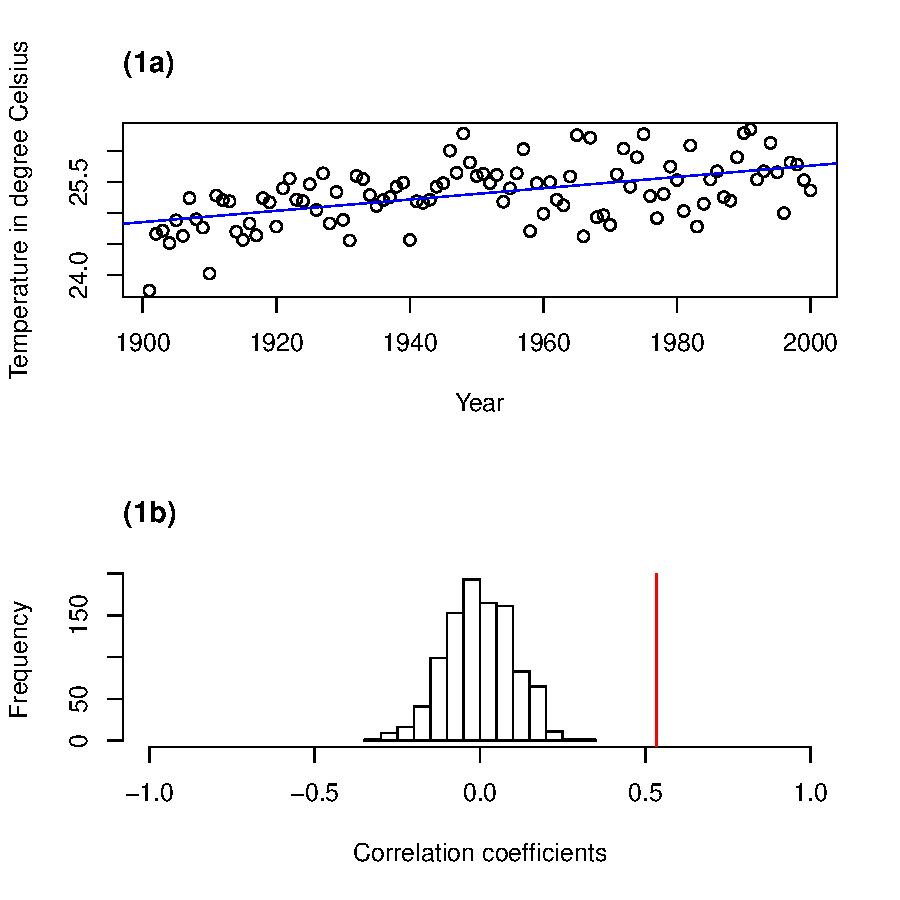
\includegraphics[width=0.5\textwidth]{fig.pdf}


{\footnotesize Fig 1: Change in temperature over year in Key West, Florida (a) and distribution of random coefficients from permutation analysis (b). Regression line is in blue and observed correlation coefficient is shown in the red vertical line.  }


\vspace{\baselineskip}

  Florida is getting warmer. 

  The correlation coefficient observed in the given year and time data is 0.533. 
  Permutation analysis shows that none of the random correlation coefficients is greater than 0.533, 
  suggesting that the asymptotic p-value is 0. The p-value of getting such a correlation by random is 0. 
  Therefore there is a significant positive correlation between year and temperature in Florida. 
  
  In Florida, temperatures of one year is significantly correlated with the next year. 


\end{document}